\documentclass[10pt,a4paper]{article}
\usepackage[latin1]{inputenc}
\usepackage{amsmath}
\usepackage{amsfonts}
\usepackage{amssymb}
\usepackage{graphicx}
\usepackage{multicol}
\usepackage{changepage}
\usepackage{float}
\usepackage{cite}
\usepackage{url}
\usepackage{imakeidx}
\makeindex

\usepackage[left=2.50cm, right=2.50cm]{geometry}
\usepackage[spanish]{babel}

\author{Axel}
\title{Portada siempre practica}

\begin{document}
%encabezado 
\pagestyle{plain}{
\pagestyle{empty}
\changepage{3cm}{1cm}{-0.5cm}{-0.5cm}{}{-2cm}{}{}{}
\noindent

%sEGIUN EL formato de sus imagenes, deben encontrar una configuracion adeacuada para ustedes
{\small
\begin{tabular}{p{0.626\textwidth} p{0.50\textwidth} }

\includegraphics[scale=0.26]{uaem.jpg} &  
\includegraphics[scale=0.3]{ico.jpg}
\end{tabular}
}

%datos de la caratula
\begin{center}
\par\vspace{2cm} %Rspacoo dejado antes del encabezado
{
\Huge\textbf{
Universidad Aut\'onoma del Estado de Mex\'ico \\[1cm] Ingenieria en Computaci\'on
}
}
\par\vspace{1.5cm}
{
\Large\textbf{ Materia: Redes Neuronales \\ Red Neuronal Feed Forward
}
}
\par\vspace{1.5cm}
{
\large\textbf{Axel Valenzuela Ju\'arez \\Profesor: Dr. Asdr\'ubal	L\'opez	Chau \\ 12 de Noviembre del 2019 } 
}

\par\vspace{1.5cm}

\end{center}
\clearpage

}

\printindex

\section{
Introducci\'on a Red Neuronal Feed Forward
}
\subsection{Red Neuronal Feed Forward}
\paragraph{
Pueden clasificarse en distintas categor\'ias.
}
\paragraph{
En las redes feedforward se empieza con un vector de entradas el cual es equivalente en magnitud al n\'umero de neuronas de la primera capa de la red, las cuales procesan dicho vector elemento por elemento en paralelo.
}
\paragraph{
La informaci\'on, modificada por los factores multiplicativos de los pesos en cada neurona, es transmitida hacia delante por la red pasando por las capas ocultas para finalmente ser procesada por la capa de salida. Es por eso que este tipo de redes reciben su nombre.
feedforward son las m\'as sencillas en cuanto a implementaci\'on y simulaci\'on, pero su desempenio es bueno para aplicaciones en los que no se requiera que la red retenga informaci\'on de eventos pasados como ayuda para evaluar eventos futuros.
 en la Fig:\ref{fig:Compuertas}
}



\begin{figure}[H]
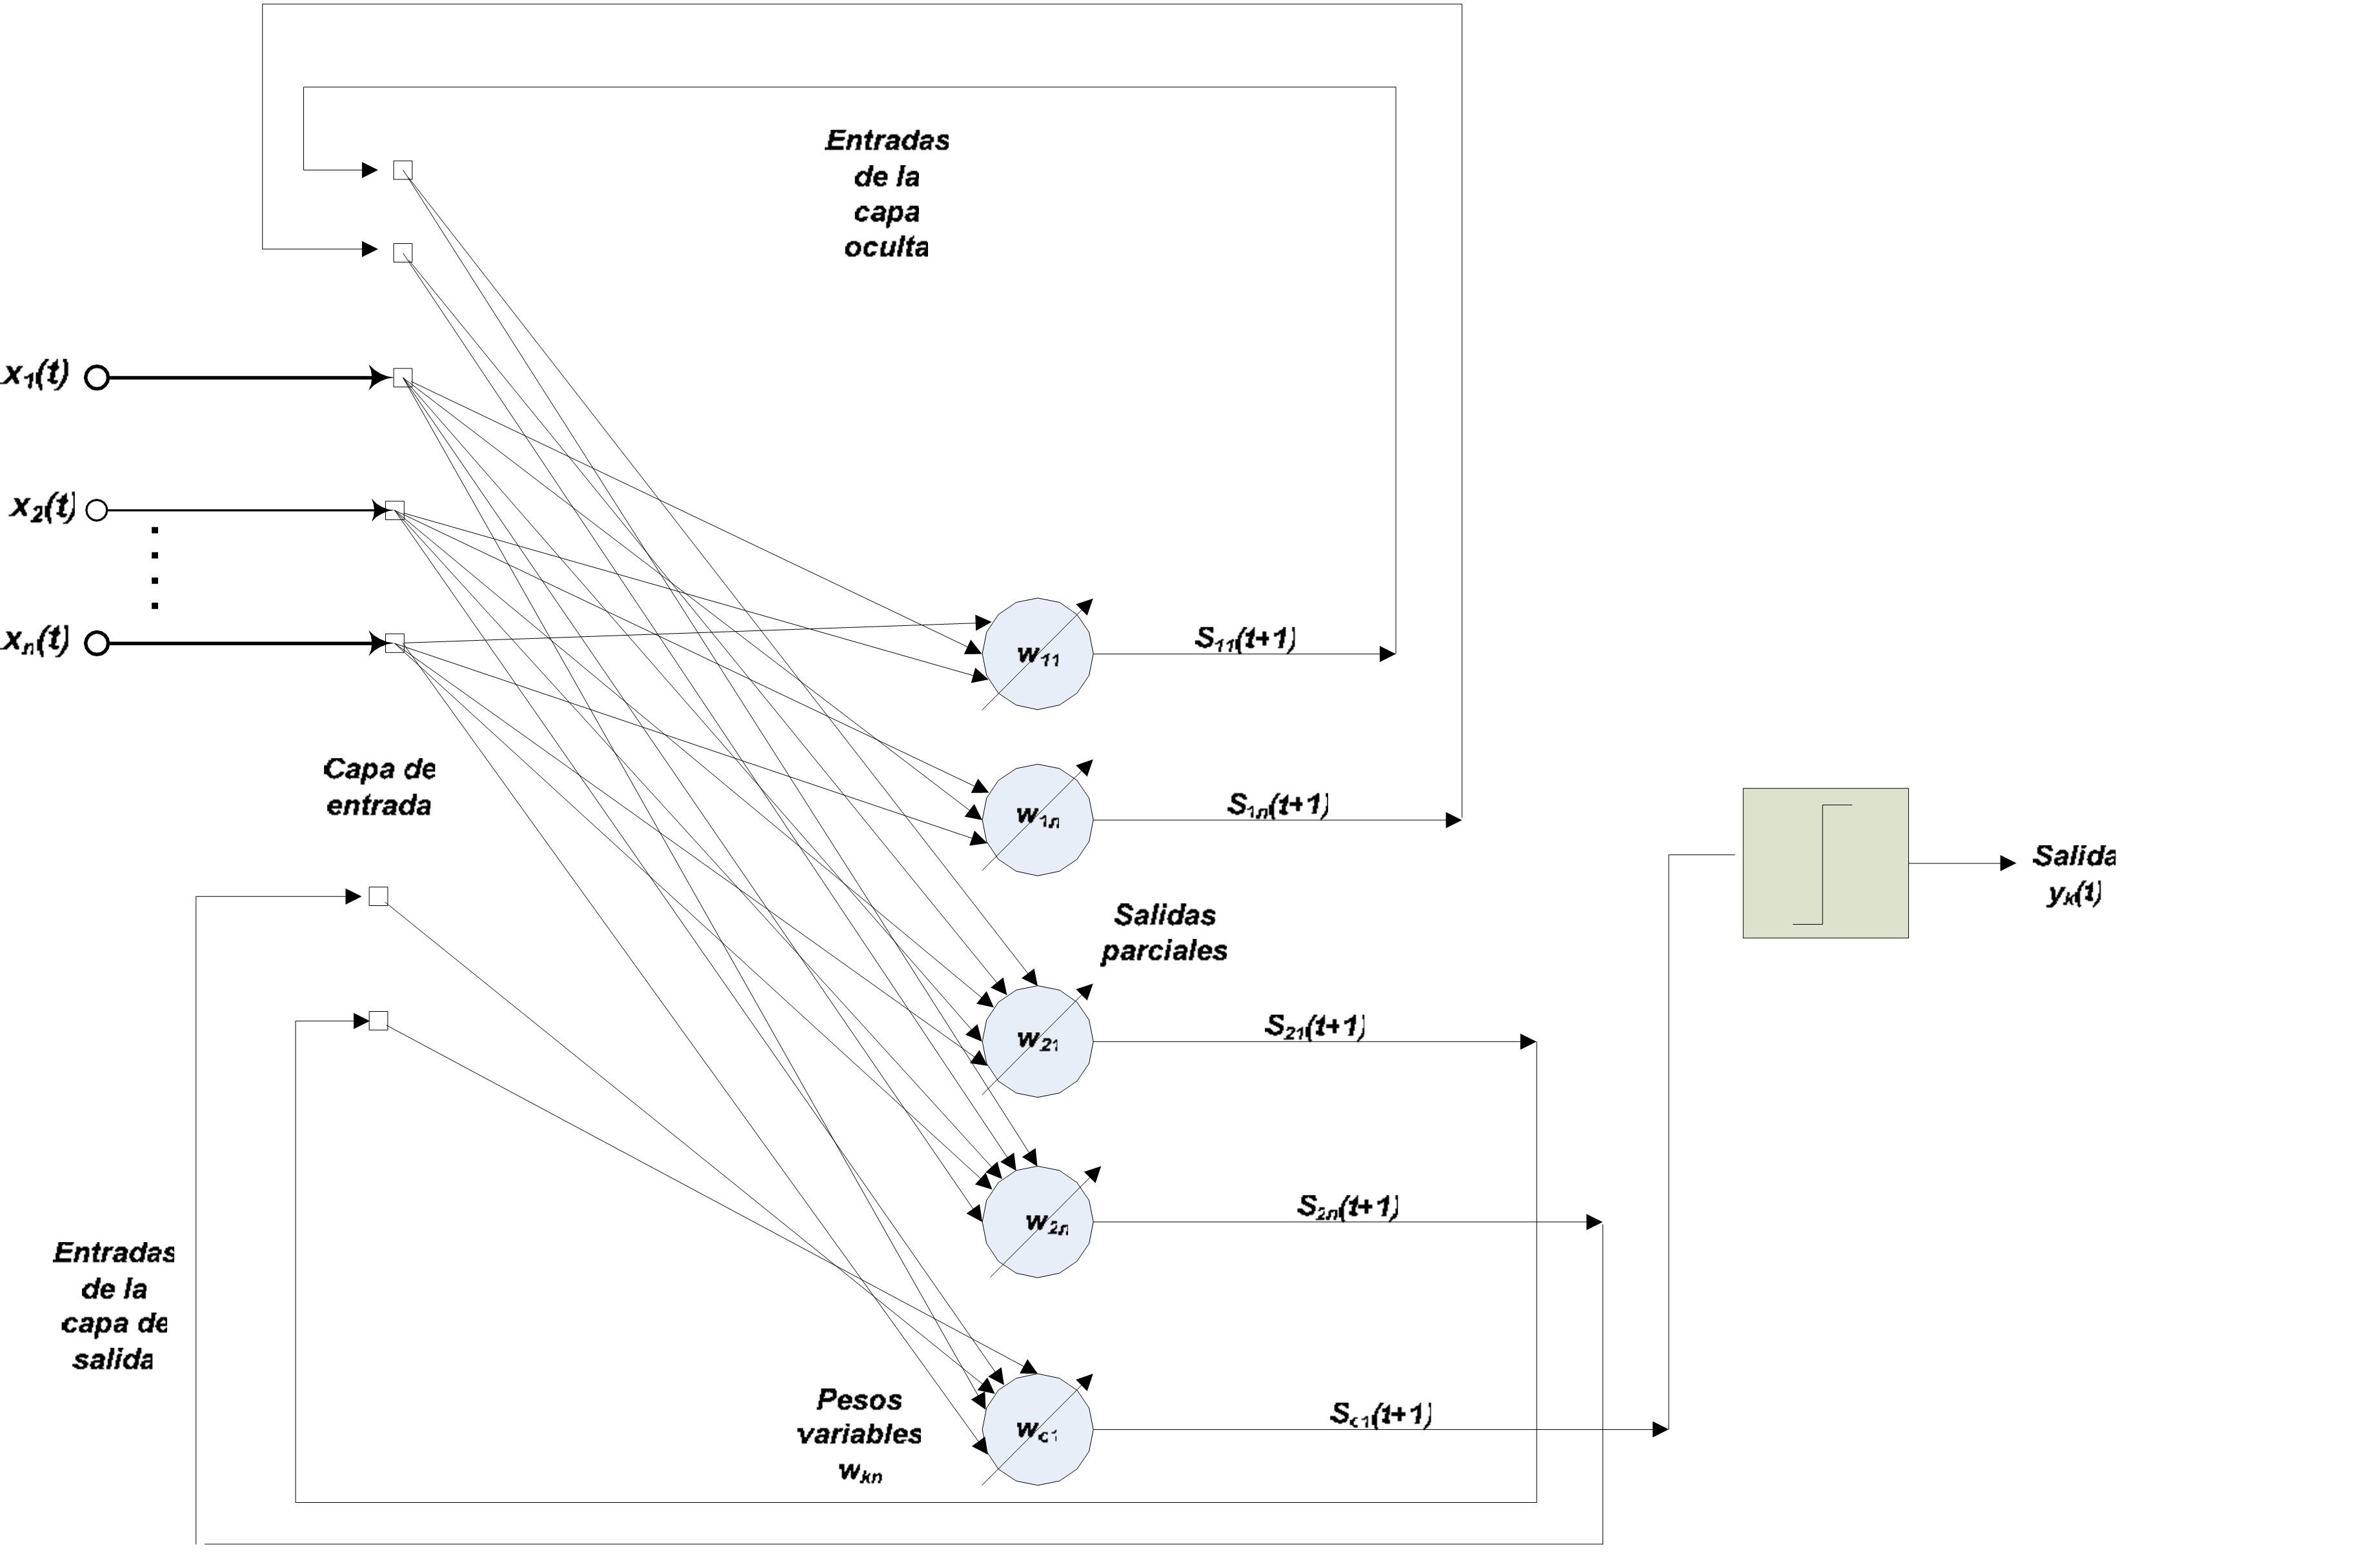
\includegraphics[scale=0.15] {neuro.png}
\caption{Red Feedforward.}
\label{fig:Compuertas}
\end{figure}


\subsection{Desarrollo}

\paragraph{El desarrollo puede ser f\'acil de entender, es una red multicapa la cual queremos ocupar en m\'ultiples casos, por lo cual se tiene que comprender el funcionamiento de una neurona anteriormente visto en otras pr\'acticas.
Se debe identificar la estructura de una red multicapa la cual est\'a compuesta por una capa de entrada, una o m\'ultiples capas ocultas y una capa de salida.
En cada una de ellas se deber\'a sacar el resultado de la red con la siguiente ecuaci\'on:
$Y=f(w^t(x))$
}

\paragraph{Se puede comenzar partiendo del codigo visto en clase de como hacer una red neuronal fija.}

\paragraph{En este caso la primer modificaci\'on sera pedir al usuario los requisitos de la practica, siendo ,N\'umero de entradas (valor entero)
,N\'umero de capas ocultas (valor entero)
,N\'umero de neuronas en cada capa oculta (lista de valores enteros) ,N\'umero de salidas (valor entero).}



\paragraph{Se crea un ciclo for el cual ayudara a crear las multiples capas que sean necesarias, se le agrego un mas 2 por la capa de entrada y salida, se usaron 3 if para determinar en que capa se encontrara el algoritmo, en la linea 25 se puede observar que se crea una matriz con n\'umeros aleatorios para las entradas, posteriormente se le agregara un 1 a la matriz.}
 \paragraph{Se creara la matriz w en la linea 28, despues se calculara la matriz transpuesta entre w y los datos de entrada asi como se le pasara los datos para ser calculados en la funcion funcAct, como se puede observar en la Fig: \ref{fig:cod1}}



\begin{figure}[H]
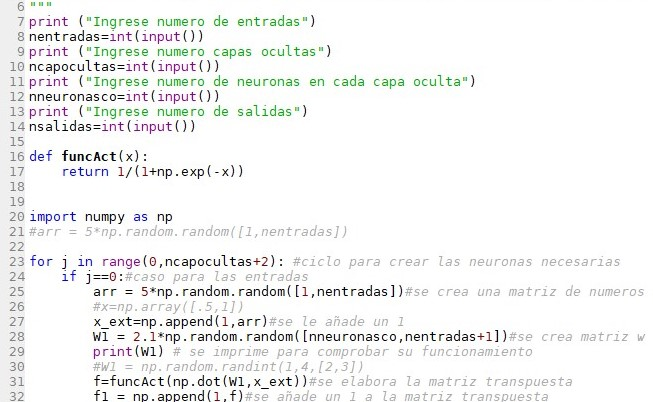
\includegraphics[scale=0.7] {cod1.jpg}
\caption{Previsualizaci\'on de Codigo.}
\label{fig:cod1}
\end{figure}
 
\paragraph{Obtendremos el resultado y se agregara un 1 a la matriz para ser ocupado posteriormente.}
\paragraph{El algoritmo pasara al caso de las capas ocultas, en esta parte del c\'odigo que comienza desde la línea 34 se realizaran los c\'alculos dependiendo el n\'umero de capas ocultas dado. El algoritmo funciona muy parecido a la primer parte , solo que en este caso se tiene que tener presente los resultados de las neuronas anteriores para ello me apoye de la variable fy obteniendo el n\'umero de filas o neuronas, a partir de ese punto el procedimiento se repite, se creara una matriz w con n\'umeros aleatorios y despu\'es se calculara la matriz transpuesta para ser pasada por la funci\'on funcAct, como se puede observar en la Fig: \ref{fig:cod2}}

\begin{figure}[H]
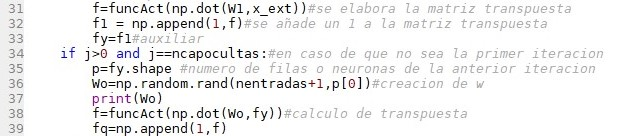
\includegraphics[scale=0.7] {cod2.jpg}
\caption{Codigo correspondiente a capa oculta.}
\label{fig:cod2}
\end{figure}

\paragraph{Para finalizar el c\'odigo pasa a la secci\'on de la capa de salida, para ello es nuevamente necesario apoyarse de una variable en este caso fq para saber la cantidad de neuronas en la anterior iteraci\'on, despu\'es de eso el algoritmo ser\'a el mismo , se calculara la matriz transpuesta y se pasara a la funci\'on funcAct para obtener el resultado final, el cual se imprimir\'a en la variable Y, como se puede observaren la Fig: \ref{fig:cod3} }

\begin{figure}[H]
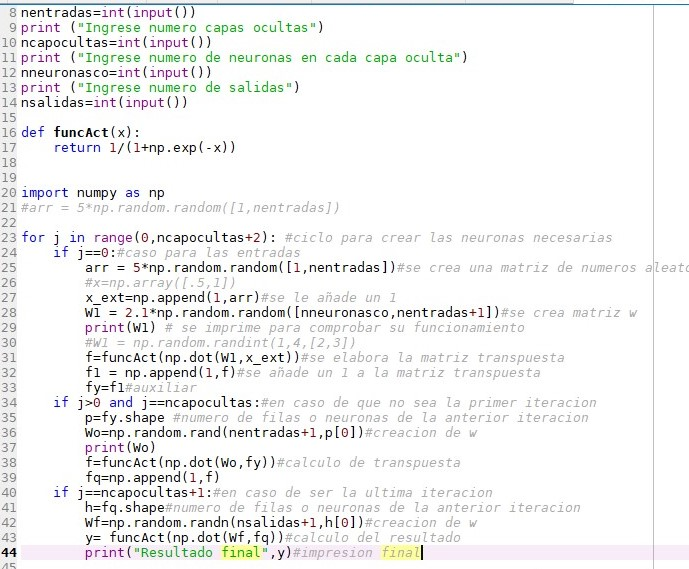
\includegraphics[scale=0.7] {cod3.jpg}
\caption{Codigo completo.}
\label{fig:cod3}
\end{figure}

\section{Pruebas Desarrolladas}

\begin{figure}[H]
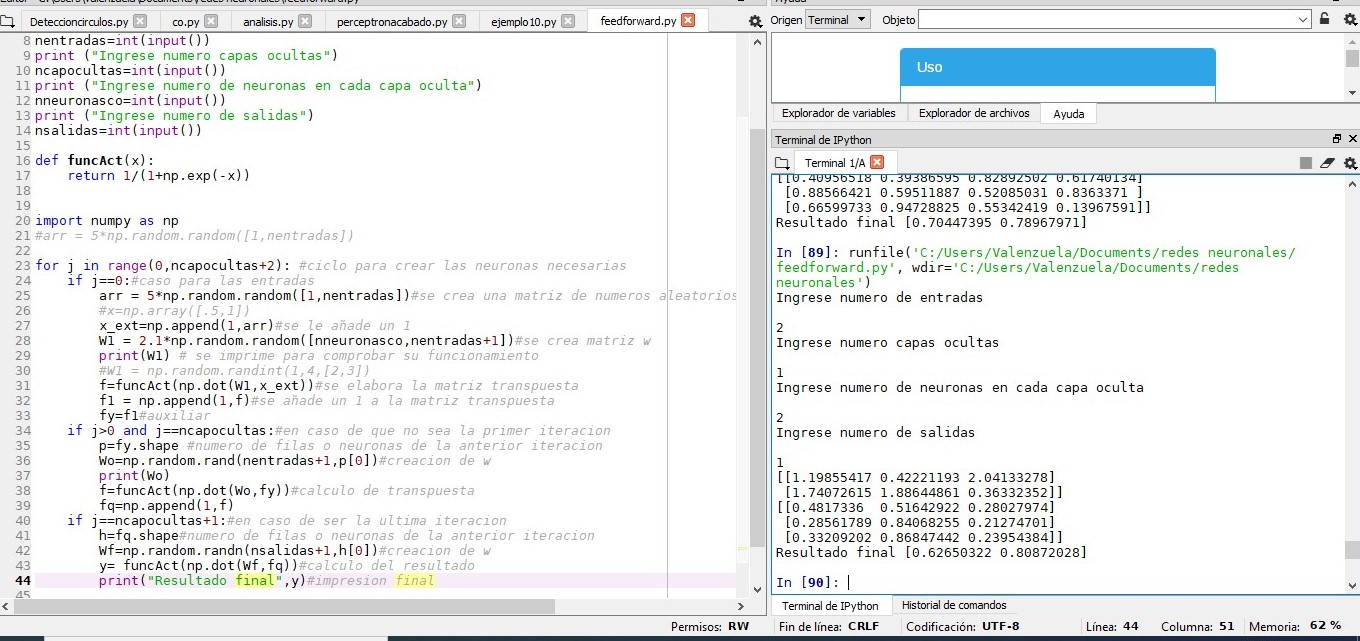
\includegraphics[scale=0.4] {p1.jpg}
\caption{Prueba 1.}
\label{fig:p1}
\end{figure}

\begin{figure}[H]
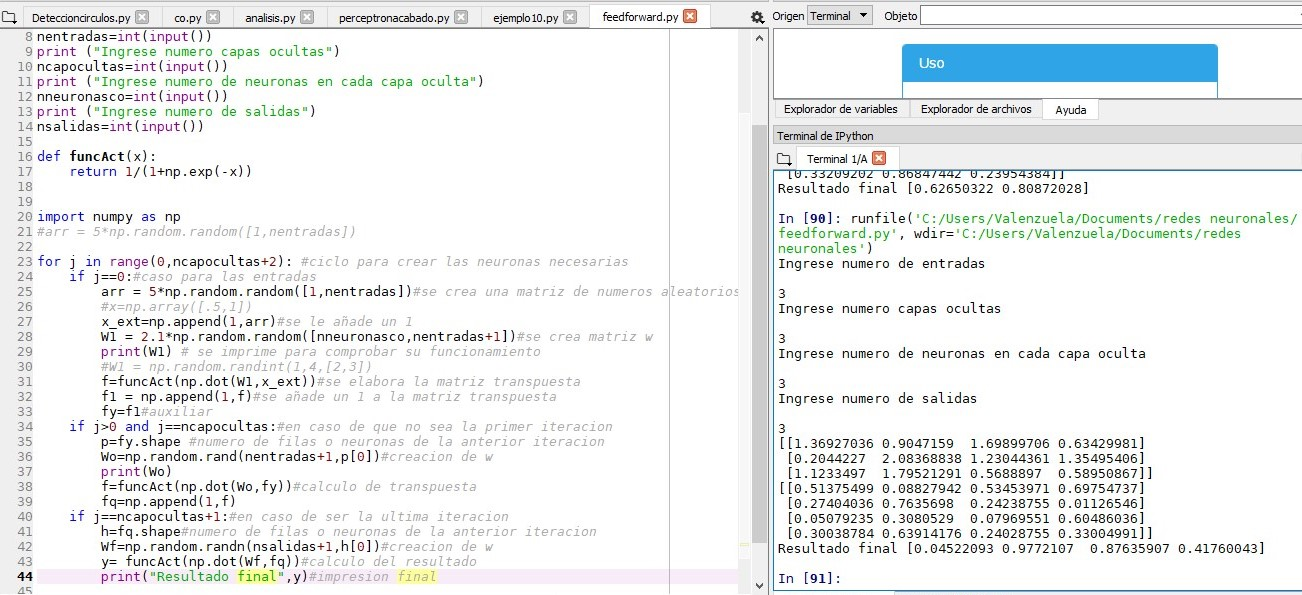
\includegraphics[scale=0.4] {p2.jpg}
\caption{Prueba 2.}
\label{fig:p2}
\end{figure}
\begin{figure}[H]
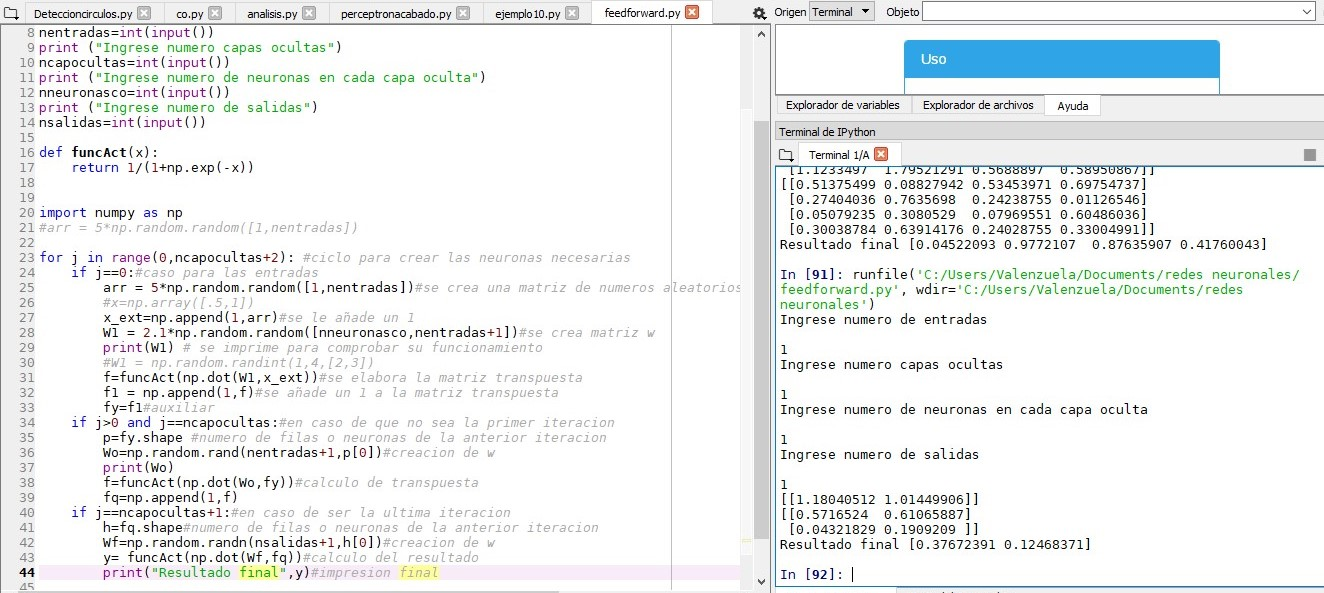
\includegraphics[scale=0.4] {p3.jpg}
\caption{Prueba 3.}
\label{fig:p3}
\end{figure}
\begin{figure}[H]
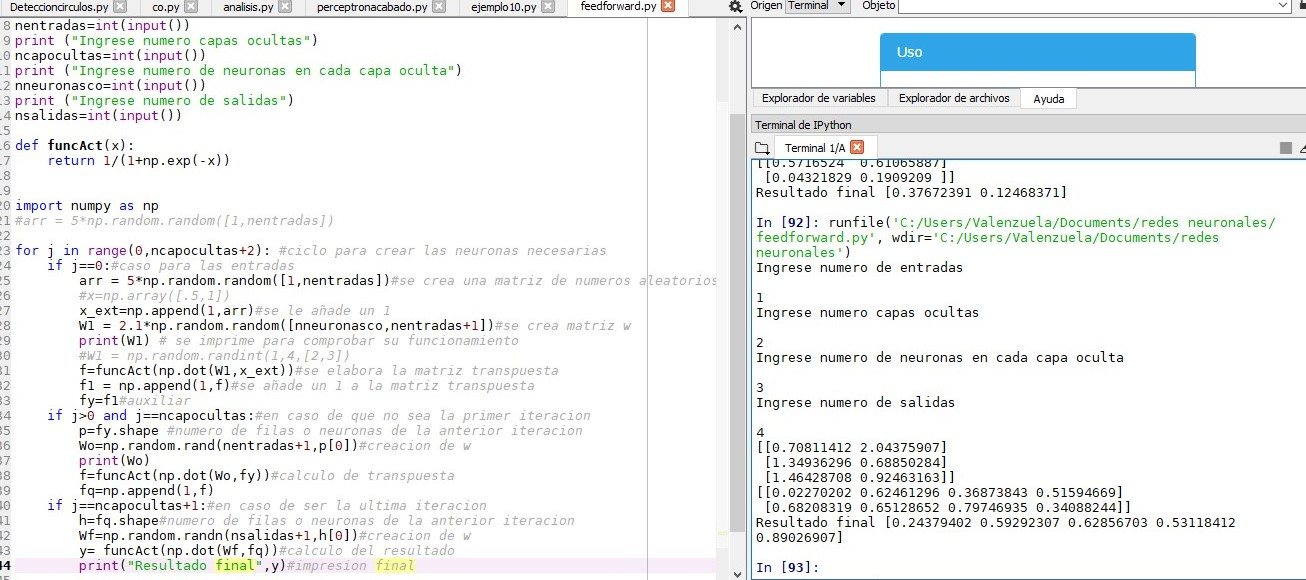
\includegraphics[scale=0.4] {p4.jpg}
\caption{Prueba 4.}
\label{fig:p4}
\end{figure}
\begin{figure}[H]
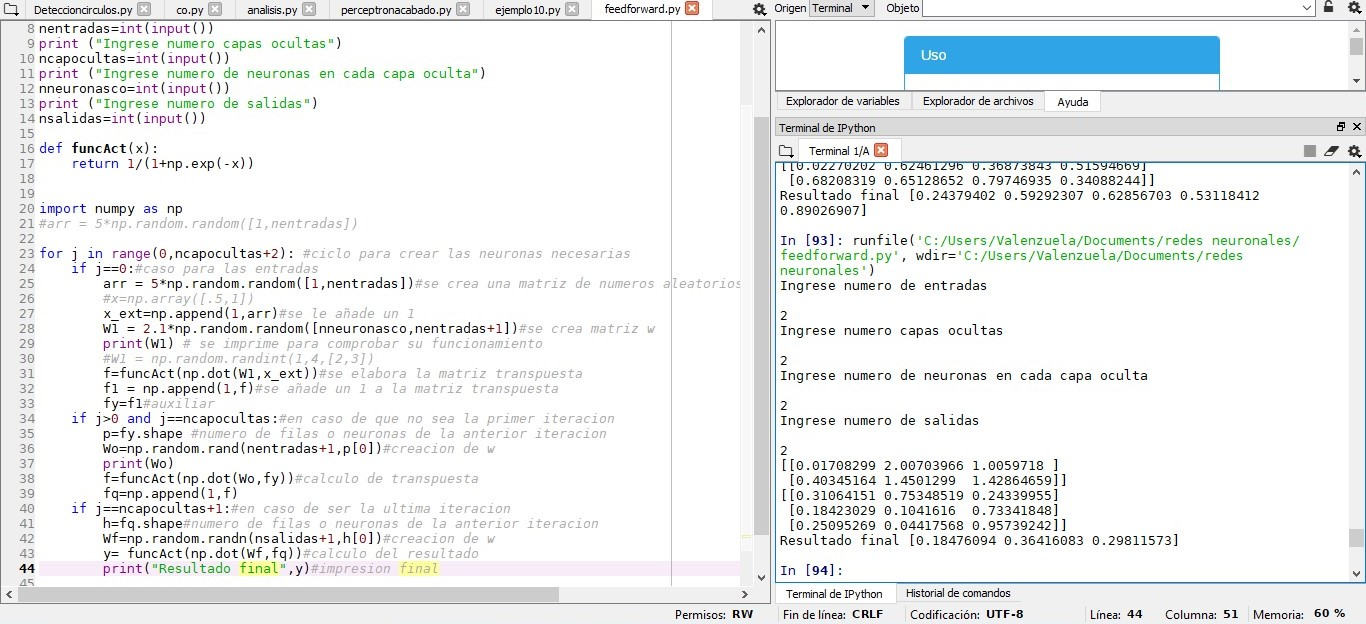
\includegraphics[scale=0.4] {p5.jpg}
\caption{Prueba 5.}
\label{fig:p5}
\end{figure}
\begin{figure}[H]
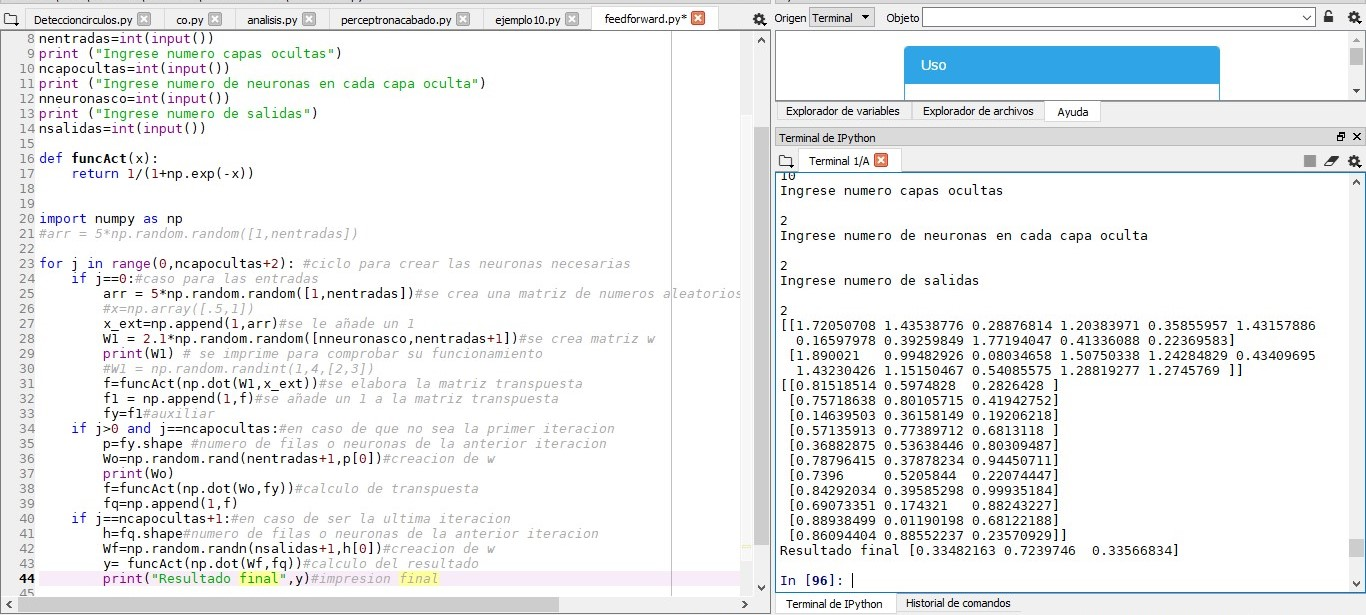
\includegraphics[scale=0.4] {p6.jpg}
\caption{Prueba 6.}
\label{fig:p6}
\end{figure}
\section{Conclusion}
\paragraph{En conclusion el algoritmo de  Feed Forward demuestra el potencial que tienen las redes multicapa, logrando analizar multiples clases y dando solucion a gran mayoria de ploblemas,  Feed Forward
es facil de programar e implementar.}
\paragraph{Es de gran utilidad conocer el funcionamiento de este algoritmo  ya que un ingeniero debe saber como funcionan las cosas para poder ser capaz de innovar y crear cosas nuevas.}

\section{Referencias}
\paragraph{L\'opez, J. P. (2014). RED NEURONAL FEEDFORWARD. Sanfandila, Qro: T\'ecnica No. 406.}
\paragraph{Ortega, J. M. (2018). APLICACI\'ON DE UNA RED NEURONAL . Creative Commons Atribuci\'on-NoComercial-CompartirIgual 3.0 Internacional.}

\end{document}
